\section{Architecture for Adjustable Monitoring}
\label{sec:dropping}

In this section, we present our hardware architecture that enables partial
monitoring for adjustable overheads. Section~\ref{sec:dropping.baseline} first
describes our baseline model for run-time monitoring while the rest of the
section describes our design.

\subsection{Baseline Architecture}
\label{sec:dropping.baseline}

% Run-time monitoring overview
\begin{figure}
  \begin{center}
    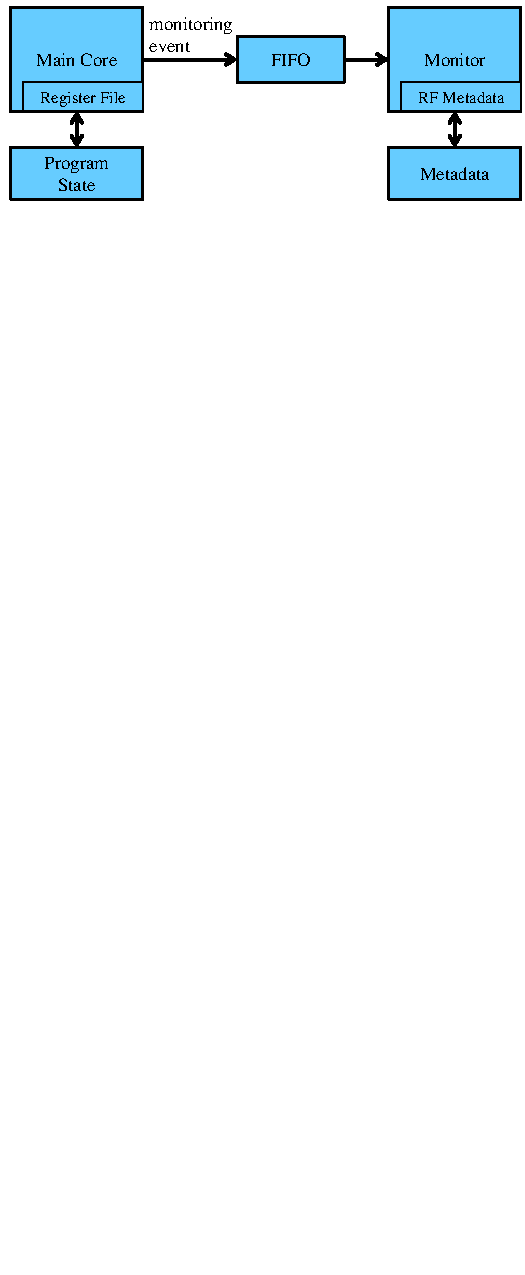
\includegraphics[width=\columnwidth]{figs/monitoring_architecture.pdf}
    \vspace{-0.2in}
    \caption{Overview of run-time monitoring architecture.}
    \label{fig:dropping.overview} 
    \vspace{-0.1in}
  \end{center}
\end{figure}

Figure~\ref{fig:dropping.overview} shows an overview of the run-time monitoring
model that is assumed in this paper.  The \emph{main program} is a computation
task that performs the original function of the system and is run on the
\emph{main core}.  On certain events during the main program, such as the
execution of certain types of instructions, the \emph{monitor} performs a
series of \emph{monitoring operations}. The monitor operates in parallel to the
main core. These events are referred to as \emph{monitoring events}. Depending
on the type of monitoring event, different monitoring operations are
executed. Information about monitoring events is sent to the monitor and buffered in a FIFO structure to decouple the
running of the main core and the monitor. If the FIFO is full, then the main
core is forced to stall on a monitoring event until a FIFO entry becomes
available. These stalls are a major source of
overhead because the monitor may take several cycles to process a single event
from the main core. 
Monitors typically maintain a set of metadata corresponding to the main
program's memory. Similarly, monitors also typically maintain a set of metadata
corresponding to the main core's register file.
%We refer to these stalls and other overheads, such as
%contention for shared resources, as \emph{monitoring overheads}. 
Monitors typically maintain metadata corresponding to each memory location
({\tt mem\_metadata[addr]}) and register ({\tt rf\_metadata[reg\_id]}) of the
main core.
If the monitor
detects an inconsistent or undesired behavior in the monitoring events, then
an error is detected. 

There are many possible monitoring schemes that can be implemented on this type
of fine-grained parallel monitoring architecture such as memory protection
\cite{mondrian-asplos02}, information flow tracking \cite{dift-asplos04,
testudo-micro08}, soft error detection \cite{argus-micro07}, data-race
detection \cite{cord-hpca06}, etc.  For example, an array bounds check (BC)
\cite{hardbound-asplos08} can be implemented in order to detect
when software attempts to read or write to a memory location outside of an
array's bounds. This can be done by associating metadata with array pointers that 
indicates the array's base (start) and bound (end) addresses. On loads or stores with the
array
pointer, the monitor checks that the memory address accessed is within the base and
bound addresses. In addition, this base and bound metadata
is propagated on ALU and memory instructions to track the corresponding array pointers.
% One example is an uninitialized memory check (UMC) where monitoring is used to
% detect when software attempts to read from a memory location that was not
% previously initialized. This can be done by forwarding each load and store
% instruction from the main core to the monitor. For every memory location, the
% monitor keeps one bit of metadata. On a store to a memory location, the monitor
% marks the corresponding metadata bit to indicate that the memory location has
% been initialized. On a load, the monitor checks that the corresponding metadata
% bit has been previously marked as initialized.

% There are multiple options for implementing programmable parallel monitors. For
% example, the Log-Based Architecture \cite{lba-isca08} uses processor cores in a
% multi-core system as monitors. The FlexCore architecture
% \cite{flexcore-micro10} instead uses an FPGA-fabric to implement the
% monitor. 
% 
% The approach we describe in this paper applies to any of these
% parallel monitors. However, for experiments, we model an FPGA-based monitor
% similar to FlexCore.  The on-chip FPGA fabric is used to implement the
% ``Monitor'' block in Figure~\ref{fig:arch.overview} while the FIFO from the
% main core and metadata cache are implemented as ASICs.

% Example monitor
\begin{figure*}
  \begin{center}
    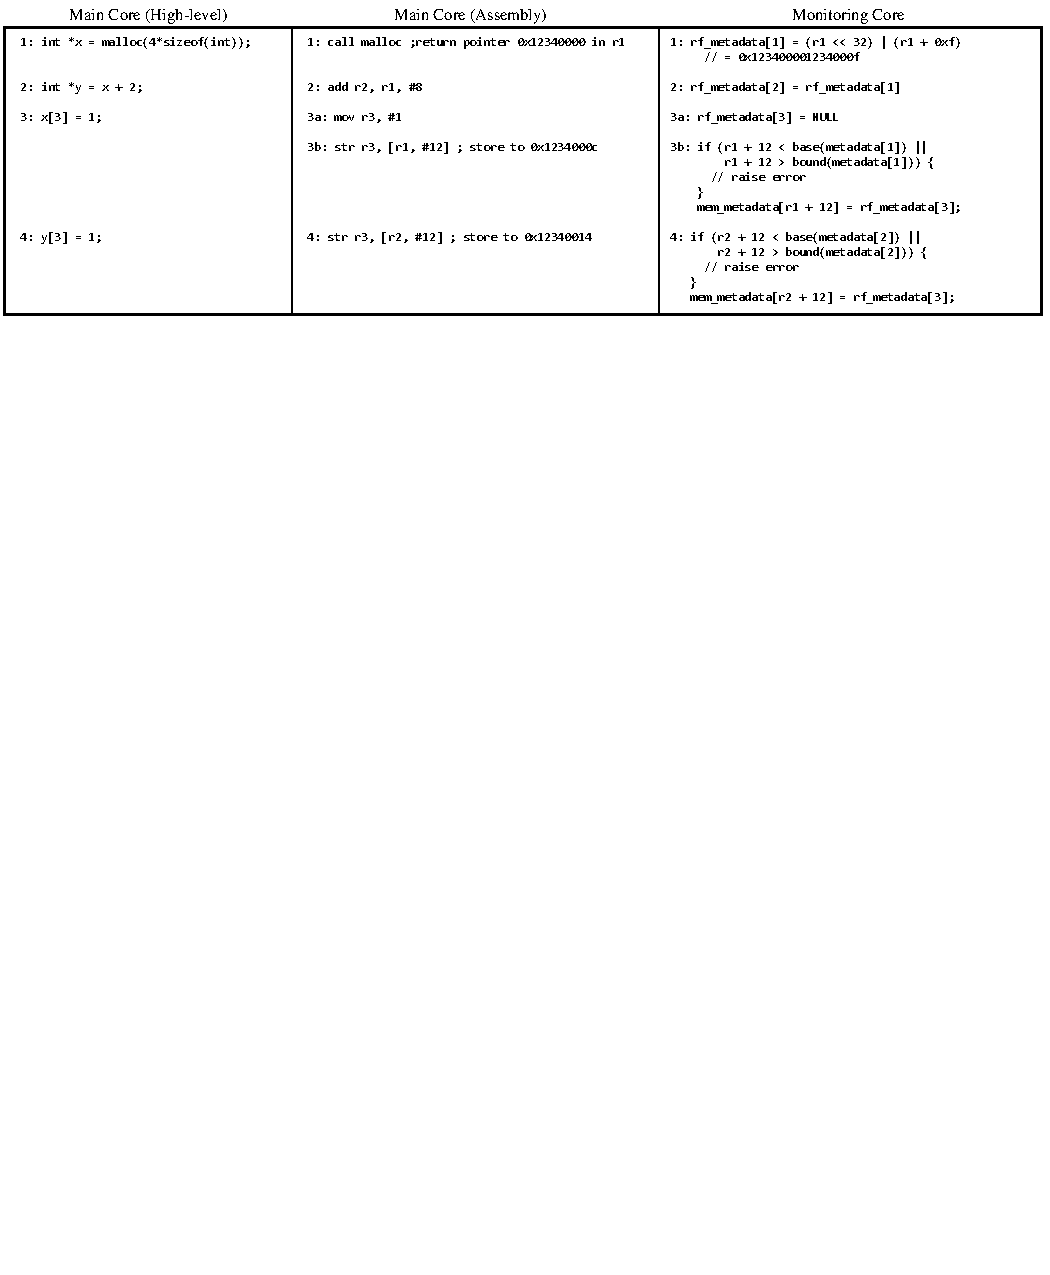
\includegraphics[]{figs/example_full.pdf}
    \vspace{-0.2in}
    \caption{Example of array bounds check monitor.}
    \label{fig:dropping.example_full}
    \vspace{-0.1in}
  \end{center}
\end{figure*} 

Figure~\ref{fig:dropping.example_full} shows an example pseudo-code segment,
its assembly level instructions, and the corresponding monitoring operations
for an array bounds check monitor. 
First, an array {\tt x} is allocated using {\tt malloc} (line 1). 
As {\tt malloc} returns the array's address in a register, the monitor
associates base and bounds metadata with the corresponding metadata. 
Next, pointer {\tt y} is set to point to the middle of array {\tt x} (line 2). 
At the assembly level, a register {\tt r2} is set to array {\tt x}'s address plus an offset.
The monitor propagates the metadata of the original pointer in {\tt r1} to the
metadata of {\tt r2}. This is to ensure that pointer {\tt y} is not used to exceed the array's bounds.
Line 3a shows setting register {\tt r3} to a constant value of 1.
When this happens,
{\tt r3}'s metadata is also reset to NULL in case it previously stored a
pointer. 
Finally, the value of {\tt r3} is written using both pointers {\tt x} and {\tt y}.
In both cases, the monitor checks whether the address that is written
to is within the bounds stored in the metadata. In the first case (line 3b), {\tt x+12}
is within the original array's bounds. No error is raised and the metadata of
{\tt r3} is propagated to the metadata of the store address. If {\tt r3} were a
pointer, than this would allow a future instruction to load the pointer and use
it to access the corresponding array or data structure. In the second case,
{\tt y+12} (line 4) corresponds to {\tt x+20} which is not within the array's bounds and
the monitor will raise an error. 

Here, we have shown the dynamic sequence of operations of the monitor.
The actual static code consists of a set of instructions to be run for each
monitored instruction type. Register and memory addresses are read from
information sent by the main core.

% \subsection{Architecture Overview}
% 
% % Overview of full architecture
% %\begin{figure}
% %  \begin{center}
% %    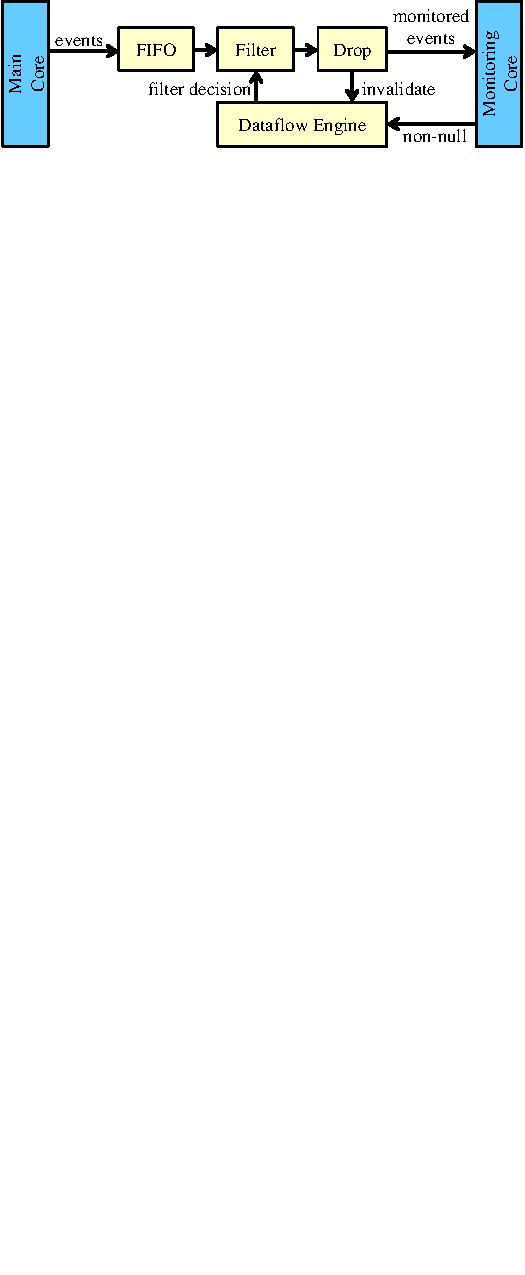
\includegraphics[width=\columnwidth]{figs/architecture_overview.pdf}
% %    \vspace{-0.2in}
% %    \caption{Block diagram of architecture for monitoring with reduced and adjustable overheads.}
% %    \label{fig:dropping.overview}
% %    \vspace{-0.1in}
% %  \end{center}
% %\end{figure}
% 
% Figure~\ref{fig:dropping.overview} shows a high-level block diagram of our
% proposed architecture for enabling partial monitoring. The basic idea is to
% insert hardware between the main core and the monitoring core to transparently
% drop monitoring events. 
% 
% There were three main challenges in designing this dropping hardware:
% \begin{enumerate}
%   \item \textbf{General:} The hardware needs to be applicable to a wide range of monitoring schemes.
%   \item \textbf{No false positives:} False positives should never occur as a result of dropping.
%   \item \textbf{Intelligent dropping:} The hardware needs to maximize the amount of useful monitoring done while staying within the overhead budget.
% \end{enumerate}
% 
% In order to reduce overheads, the ``Drop'' module decides when monitoring event
% should be skipped.  This decision of when to drop and which monitoring events
% to dropped is discussed in more detail in Section~\ref{sec:policies}.
% 
% When an event is dropped, metadata needs to be invalidated in order to prevent
% false positives. This is done using a hardware dataflow engine.
% Sections~\ref{sec:dropping.false_neg_pos} and
% \ref{sec:dropping.prevent_false_pos} discuss these false positive issues and
% the dataflow engine in detail. 
% 
% In addition, we can use the dataflow engine to filter out monitoring operations
% that would be operating on invalid metadata. This maximizes the useful
% monitoring that is done by the monitoring core.
% Section~\ref{sec:dropping.filter} talks about how this is done using
% information from the dataflow engine.

\subsection{Effects of Dropping Monitoring}
\label{sec:dropping.false_neg_pos}

Our goal is to drop some monitoring operations in order to reduce the overheads
of run-time monitoring. This dropping can affect the functionality of the
monitoring schemes. There are three possible outcomes for dropping a
monitoring operation. The first is that there is no difference in operation
from the original execution. For example, if we drop line 3b from our array
bounds check example (Figure~\ref{fig:dropping.example_full}), then the
check on accessing {\tt x+12} is skipped. However, this is a valid access and so
skipping the check does not change anything.

On the other hand, if the monitoring for accessing memory location {\tt y+12} on
line 4 is skipped, then
a false negative occurs. Originally, the monitor would catch this access as an
out-of-bounds access and raise an error. However, if the monitoring operation
for this is dropped, then the error is not detected. This is the trade-off that
we make in order to reduce overheads. That is, instead of either 100\% coverage
with all the associated overheads or no coverage and no overheads, we 
enable middle points of partial coverage with some fraction of the full
overheads.

The final possible outcome of dropping a monitoring operation is a false positive. 
For example, suppose the monitoring for
line 1 is dropped, causing the bound information for pointer {\tt x} to never
be set. The result is that when the access using {\tt x} is checked on line 3b,
an error will be raised. This creates a false positive where an error is
incorrectly raised. Although false negatives are part of the trade-off we make
to reduce overheads, we need to prevent false positives.

\subsection{Invalidation for Preventing False Positives}
\label{sec:dropping.prevent_false_pos}

% In analyzing various monitoring schemes, we found that monitoring operations
% are primarily of two types: \emph{checks} and \emph{metadata updates}. Monitors
% \emph{check} certain properties to ensure correct main program execution (lines
% 3b-4 of Figure~\ref{fig:monitoring.example_full}) and they \emph{update} metadata
% for bookkeeping (lines 1-3a of Figure~\ref{fig:monitoring.example_full}). Skipping
% a check operation can only cause false negatives and will never cause a false
% positive (see Figure~\ref{fig:dropping.example_no_error} and
% Figure~\ref{fig:dropping.example_false_negative}). Therefore, we may simply
% skip a check operation. Skipping an update operation can cause false
% negatives but may also cause false positives (see
% Figure~\ref{fig:dropping.example_false_positive}). 

% Example with invalidation
\begin{figure*}
  \begin{center}
    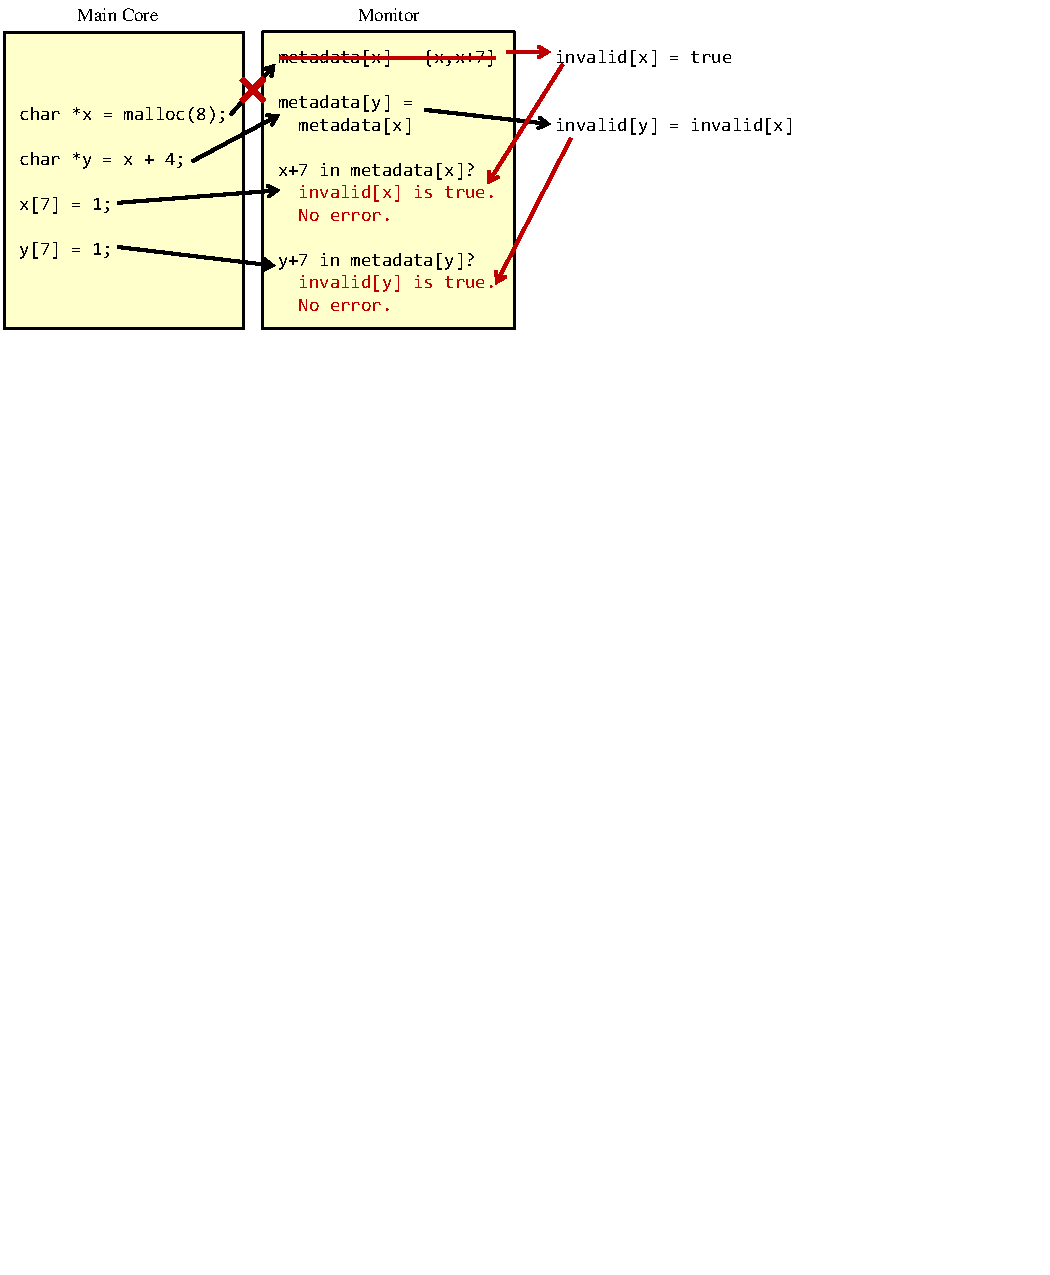
\includegraphics[]{figs/example_invalid.pdf}
    \caption{Example of using invalidation information to prevent false positives.}
    \label{fig:dropping.example_invalid}
    \vspace{-0.1in}
  \end{center}
\end{figure*}

The key cause of false positives is dropping monitoring operations that update
metadata. Dropping monitoring operations that check for an error (such as the check
for line 4 in Figure~\ref{fig:dropping.example_full}) can only cause
false negatives but will never cause false positives. On the other hand,
skipping monitoring operations that update metadata can lead to false positives
and false negatives.
Essentially, when an update operation is skipped, we can no longer trust the
corresponding metadata. Thus, our general approach for preventing false
positives is to add a 1-bit flag to each metadata in order to mark these
metadata as
invalid. Furthermore, this invalidation information is propagated in the same
way that metadata is. Figure~\ref{fig:dropping.example_invalid}
shows an example of associating invalid flags with metadata. In the example, no
monitoring operations are dropped. However, suppose that the monitoring for
line 1 is dropped. In this case, {\tt rf\_invalid[1]} will be marked as {\tt
true}. Thus, when line 3 is reached, the monitoring event is dropped
since {\tt rf\_invalid[1]} is marked as true. Note that in this case, line 2
also propagates this invalid flag to {\tt rf\_invalid[2]} and causes the check
performed on line 4 to also be dropped. This is necessary because an error
would have been raised even if the access on line 4 was in bounds.

\subsection{Dataflow Engine for Preventing False Positives}
\label{sec:dropping.arch}

% Dataflow engine high-level
\begin{figure}
  \begin{center}
    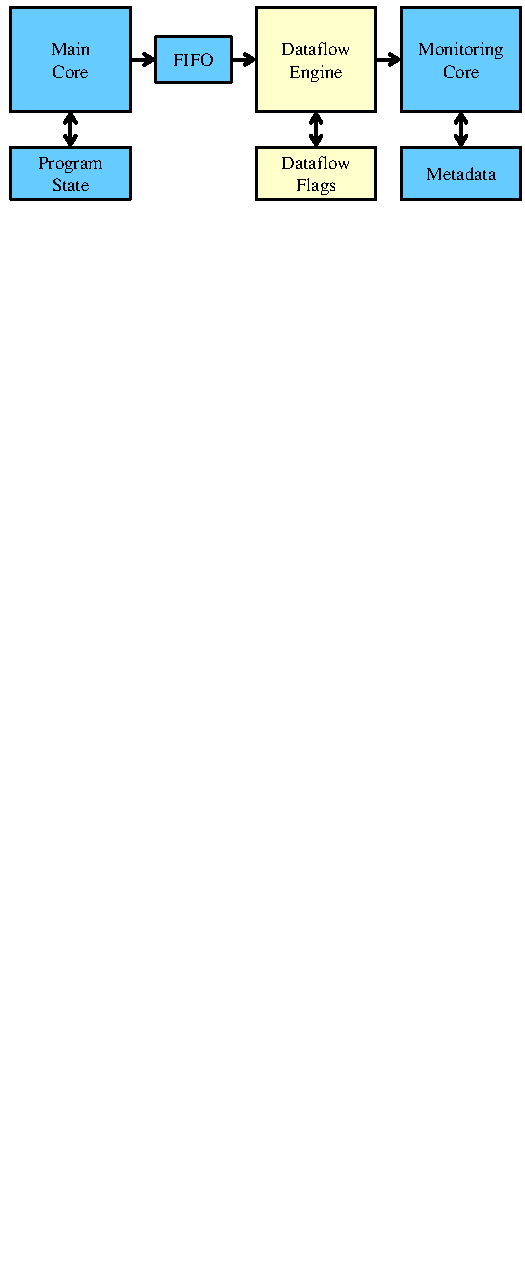
\includegraphics[width=\columnwidth]{figs/dataflow_overview.pdf}
    \caption{Hardware support for dropping.}
    \label{fig:dropping.dataflow_overview}
    \vspace{-0.1in}
  \end{center}
\end{figure}

Although the functionality of dropping and invalidation could be implemented on
the monitor, this is unlikely to be much faster than performing the full monitoring
operations.
Instead, in order to efficiently support dropping monitoring events and to prevent false
positives, we propose to insert a hardware module between the main core and
monitor (see Figure~\ref{fig:dropping.dataflow_overview}). 
This module handles the invalidation operations shown in the middle column of
Figure~\ref{fig:dropping.example_invalid}.
There are two operations that are done for handling invalidation information:

\begin{enumerate}
  \item Propagate invalid flags, following the dataflow of metadata.
  \item Filter out monitoring operations based on invalid flags.
\end{enumerate}

% Detailed architecture of dataflow engine
\begin{figure*}
  \begin{center}
    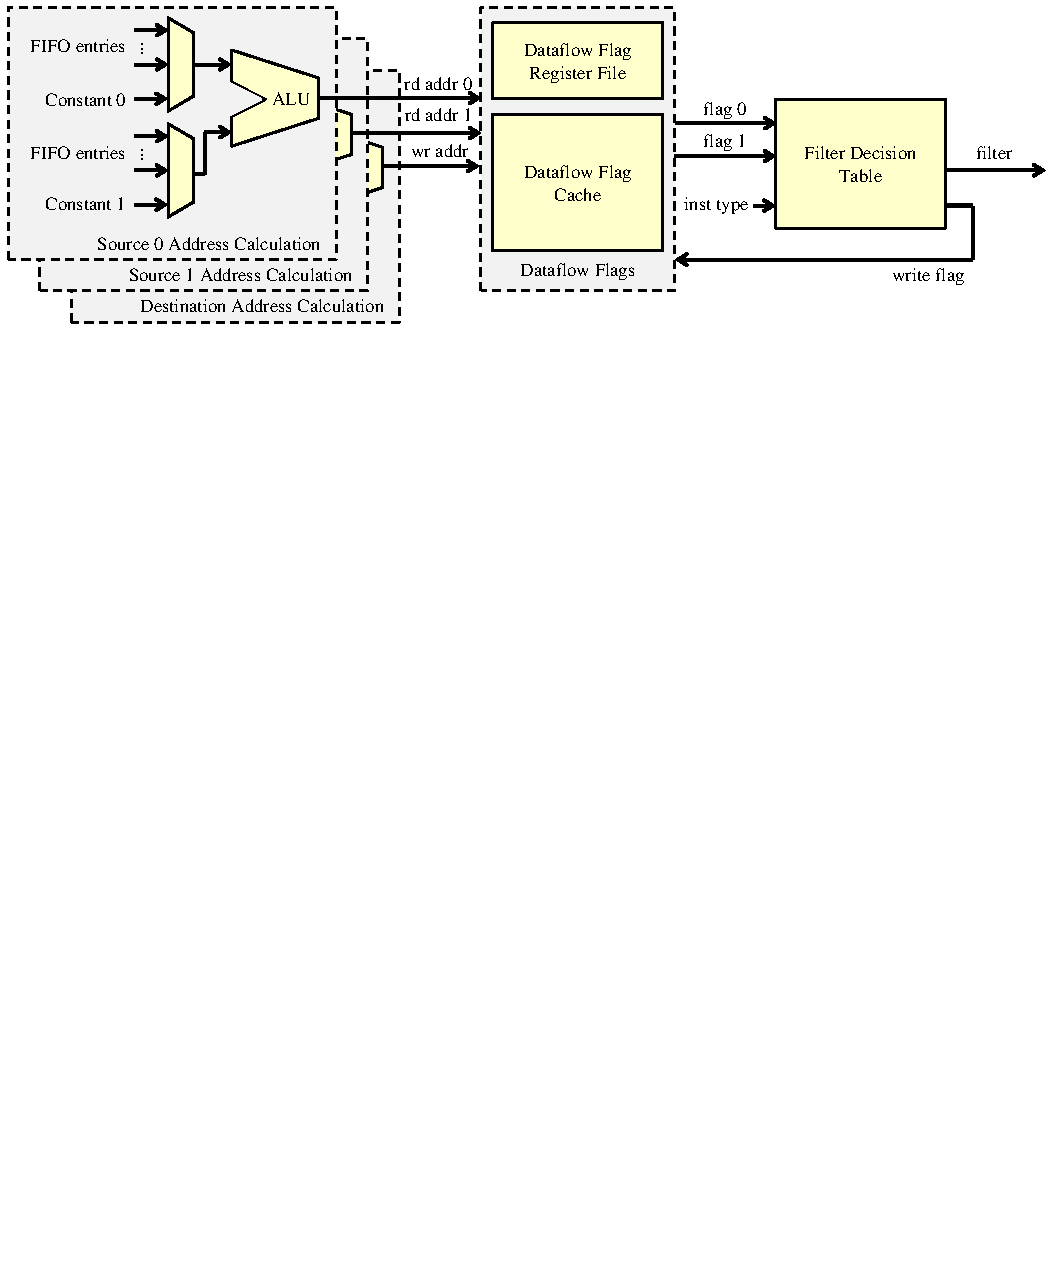
\includegraphics[]{figs/dataflow_architecture.pdf}
    \vspace{-0.2in}
    \caption{Hardware architecture of the dataflow engine.}
    \label{fig:dropping.dataflow} 
    \vspace{-0.1in}
  \end{center}
\end{figure*}

Thus, the hardware acts effectively as a dataflow tracking engine in order to
track a 1-bit invalid flag per metadata. Figure~\ref{fig:dropping.dataflow} shows a detailed block
diagram of this hardware module. The dataflow engine uses two address
calculation units to read in up two invalid flags. These source invalid flags
are used to decide whether a monitoring event should filtered. A third address
calculation unit is used to optionally specify a target to propagate the
invalidation information. The module includes a register file to store invalid
flags corresponding to register file metadata. In addition, it uses a small
memory-backed cache to handle invalid flags corresponding to memory metadata.

Since different monitoring operations are performed based on instruction type,
the dataflow engine is also configured based on instruction type. The source
and operation of the address generation units are set based on instruction
type. Note that the address calculation units also take information from the
monitored event as inputs. Thus, in the same way that the monitor selects
metadata based on register indices or memory address of the specific monitoring
event, the dataflow engine also reads the appropriate flags. In addition, the
filter decision table is configured based on instruction type to decide what
combination of input flags will lead to a filtered event and whether
propagation is required.

% Monitoring schemes typically keep metadata corresponding to the main core's
% register file as well as the main core's memory space. Similarly, the dataflow
% engine uses an on-chip register file to store flags for register file metadata.
% In addition, a set of flags are stored that correspond to memory metadata.
% These memory metadata flags are accessed through a cache and backed to main
% memory. All flags are initialized as valid when the system starts. 

% Address calculation and configuration
% On a monitoring event, the dataflow engine reads in up to two flags in order to
% determine whether the event can be filtered.  The flags to be read in typically correspond to the source
% operands of the monitored instruction. For example, on a load, the dataflow
% engine will typically read in the flags corresponding the memory location
% accessed.
% However, the architecture is designed such that the address of flags to be read
% is calculated dynamically and can be configured depending on the monitoring
% scheme. Specifically, there exists a configuration table that outputs a set of
% control signals depending on the instruction type of the monitoring event.
% These control signals are used to control a pair of address calculation units which each
% contain a simple ALU. The inputs to the ALU are information from the monitored
% event and a constant that is specified from the configuration table. One common
% use of this address calculation is to transform addresses from byte-addressed
% to word-addressed by right shifting the passed memory address by 2 bits.

% \subsection{Filtering Invalid Events}
% \label{sec:dropping.filter}
% 
% % Filtering decision
% The decision of whether an event can be filtered out is determined using a
% lookup table. This filter decision table is configured by the monitoring scheme
% on system initialization. The lookup table determines whether an event can be
% filtered out based on the pair of input flags read and the instruction type of
% the monitored event.
% For example, on an ALU instruction, if both of the source operand flags
% indicate that the corresponding metadata is null, then typically the instruction can be
% filtered out. Similarly, on an ALU instruction, if either of the source operand
% flags indicate that their corresponding metadata is invalid, then the
% instruction can also be filtered out. This filter decision is sent to the
% ``Filter'' block shown in Figure~\ref{fig:dropping.overview} which will simply pop
% filtered entries from the FIFO and not forward them. If an entry is not
% filtered, then this Filter block will pop the monitoring event entry from the
% FIFO and forward it along the datapath.
% 
% % Propagating flag information
% Finally, when an event is filtered out, it is necessary to propagate the flag
% information for the filtered event. In addition to the decision of whether to
% filter an event, the filter decision table also includes information about
% whether the destination flag should be written to and what value should be
% written to it. A third address calculation unit generates the write address for
% this destination flag. For example, for an ALU instruction, this will
% correspond to the destination register of the ALU instruction. If this ALU
% instruction is filtered out due to having a pair of null source operands, then
% the filter decision table will indicate that the destination register's
% corresponding flag should also be marked as null. 

% Flags are marked as invalid when a monitoring event is dropped due to
% insufficient overhead budget. Thus, whenever a monitoring event is dropped, the
% dropping hardware indicates this to the dataflow engine. The dataflow engine's
% write address is configured for the appropriate destination flag. When it
% receives an invalidation signal from the dropping hardware, the
% dataflow engine marks this destination flag as invalid.


\subsection{Filtering Null Metadata}
\label{sec:dropping.null_filtering}

% Null filtering code example
\begin{figure}
  \begin{center}
    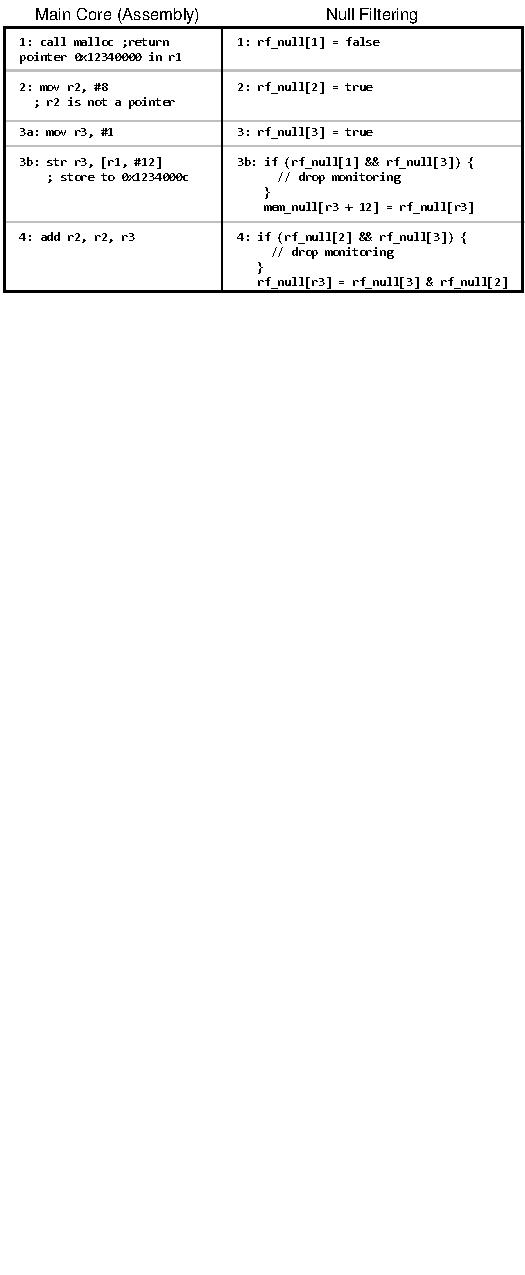
\includegraphics[width=\columnwidth]{figs/example_null_filtering.pdf}
    \vspace{-0.2in}
    \caption{Example of using information about null metadata to filter monitoring events.}
    \label{fig:dropping.example_null} 
    \vspace{-0.1in}
  \end{center}
\end{figure}

One way to reduce the number of monitoring events that must be handled by the
monitor is to filter out monitoring events that correspond to operating on null
metadata. Null metadata corresponds to events that
are not relevant to the monitor. For example, Hardbound
\cite{hardbound-asplos08} filters out operations on non-pointer (i.e., no base
and bounds metadata) instructions since it is not relevant to array bounds
checking. More recently, FADE \cite{fade-hpca14} has been proposed as a general
hardware module to perform this null metadata filtering for a variety of
monitoring schemes. 

Figure~\ref{fig:dropping.example_null} shows an example of how this null filtering operates.
Here, the main core's code has been slightly modified from
Figure~\ref{fig:dropping.example_full} and {\tt r2} on line 2 is no longer set as an array pointer.
Without null metadata filtering, the instructions for lines 2 and 4 would be
forwarded to the monitor since the system does not know whether {\tt r2}
contains a pointer address or not. However, if we use a flag to mark {\tt r2}
as null when it is loaded with a constant, then we can propagate this null
information and filter out monitoring for lines 2 and 4.

The operations performed by null filtering are almost identical to the
operations needed for invalidation shown in
Figure~\ref{fig:dropping.example_invalid}. Instead of taking a logical OR of the
source invalid flags to determine whether monitoring can be skipped, null
metadata filtering takes a logical AND of the source null flags.
Thus, we can easily enable this null metadata filtering on our architecture by
extending the dataflow flags to be two bits wide. One bit is used to
keep track of invalidation information while the second bit is used to keep
track of null information. All flags are initialized to null and the filter
decision table is extended with the propagation and filtering decision rules
for null metadata filtering.
The results is a single hardware design that provides enables both partial
monitoring and null metadata filtering.


